% Arquivo LaTeX de exemplo de dissertação/tese a ser apresentada à CPG do IME-USP
%
% Criação: Jesús P. Mena-Chalco
% Revisão: Fabio Kon e Paulo Feofiloff
% Adaptação para UTF8, biblatex e outras melhorias: Nelson Lago
%
% Except where otherwise indicated, these files are distributed under
% the MIT Licence. The example text, which includes the tutorial and
% examples as well as the explanatory comments in the source, are
% available under the Creative Commons Attribution International
% Licence, v4.0 (CC-BY 4.0) - https://creativecommons.org/licenses/by/4.0/


\documentclass[a4paper,12pt,twoside,brazilian,english]{book}
\usepackage{style/imegoodies}
\usepackage[thesis]{style/imelooks}
\graphicspath{{figuras/},{fig/},{logos/},{img/},{images/},{imagens/}}

% Comandos rápidos para mudar de língua:
% \en -> muda para o inglês
% \br -> muda para o português
\babeltags{br = brazilian, en = english}

%%%%%%%%%%%%%%%%%%%%%%%%%%%%%%%%%%%%%%%%%%%%%%%%%%%%%%%%%%%%%%%%%%%%%%%%%%%%%%%%
%%%%%%%%%%%%%%%%%%%%%%%%%%%%%%%%%% METADADOS %%%%%%%%%%%%%%%%%%%%%%%%%%%%%%%%%%%
%%%%%%%%%%%%%%%%%%%%%%%%%%%%%%%%%%%%%%%%%%%%%%%%%%%%%%%%%%%%%%%%%%%%%%%%%%%%%%%%

\addbibresource{bibliografia.bib}

\babelhyphenation{documentclass latexmk soft-ware clsguide}
\babelhyphenation[brazilian]{Fu-la-no}
\babelhyphenation[english]{what-ever}

\title{Rainbow title}[Rainbow subtitle]
\translatedtitle{Arco-iris titulo}[Arco-iris subtítulo]

\author[fem]{Nathan Luiz, Willian Mori}

\def\profa{Prof\kern.02em.\kern-.07emª\kern.07em}
\def\dra{Dr\kern-.04em.\kern-.11emª\kern.07em}

\orientador[fem]{\profa{} \dra{} Yoshiko Wakabayashi (TODO: em ingles)}

\banca{
  \profa{} \dra{} Fulana de Tal (orientadora) -- IME-USP [sem ponto final],
  % Em inglês, não há o "ª"
  %Prof. Dr. Fulana de Tal (advisor) -- IME-USP [sem ponto final],
  Prof. Dr. Ciclano de Tal -- IME-USP [sem ponto final],
  \profa{} \dra{} Convidada de Tal -- IMPA [sem ponto final],
}
\tipotese{
  tcc,
  programa={Computer Science},
}
\defesa{
  local={São Paulo},
  data=1999-11-11, % YYYY-MM-DD
}
\direitos{CC-BY}
\fichacatalografica{}

%%%%%%%%%%%%%%%%%%%%%%%%%%%%%%%%%%%%%%%%%%%%%%%%%%%%%%%%%%%%%%%%%%%%%%%%%%%%%%%%
%%%%%%%%%%%%%%%%%%%%%%% AQUI COMEÇA O CONTEÚDO DE FATO %%%%%%%%%%%%%%%%%%%%%%%%%
%%%%%%%%%%%%%%%%%%%%%%%%%%%%%%%%%%%%%%%%%%%%%%%%%%%%%%%%%%%%%%%%%%%%%%%%%%%%%%%%

\begin{document}

%%%%%%%%%%%%%%%%%%%%%%%%%%% CAPA E PÁGINAS INICIAIS %%%%%%%%%%%%%%%%%%%%%%%%%%%%

\frontmatter
\pagestyle{plain}
\onehalfspacing
\maketitle

%%%%%%%%%%%%%%%% DEDICATÓRIA, AGRADECIMENTOS, RESUMO/ABSTRACT %%%%%%%%%%%%%%%%%%

\begin{dedicatoria}
\end{dedicatoria}

\pagenumbering{roman}

\chapter*{Agradecimentos}
\epigrafe{Do. Or do not. There is no try.}{Mestre Yoda}

%%%%%%%%%%%%%%%%%%%%%%%%%%% LISTAS DE FIGURAS ETC. %%%%%%%%%%%%%%%%%%%%%%%%%%%%%

\tableofcontents

%%%%%%%%%%%%%%%%%%%%%%%%%%%%%%%% CAPÍTULOS %%%%%%%%%%%%%%%%%%%%%%%%%%%%%%%%%%%%%

\mainmatter
\singlespacing

\pagestyle{mainmatter}
%!TeX root=../tese.tex
%("dica" para o editor de texto: este arquivo é parte de um documento maior)
% para saber mais: https://tex.stackexchange.com/q/78101

\chapter{Introduction}

O problema estudado neste artigo é relativamente recente, embora suas origens remontem a conceitos clássicos. 
Em 1978, Caccetta e Häggkvist formularam a conjectura de que todo dígrafo de ordem $n$ com grau 
mínimo $d$ possui um circuito direcionado de tamanho no máximo $\lceil n/d \rceil$. Essa 
conjectura marcou o início de investigações sobre circuitos em grafos com restrições de grau.

Quase quatro décadas depois, em 2017, Ron Aharoni, do Departamento de Matemática do Technion, 
propôs uma versão mais forte dessa conjectura utilizando a versão Rainbow. Sua conjectura
afirma que, dado um grafo $G$ de ordem $n$ com arestas coloridas em $n$ cores, onde cada cor 
aparece em no máximo $r$ arestas, existe um circuito rainbow de tamanho no máximo $\lceil n/r \rceil$.

Em 2019, Felix Joos, professor na Universidade de Heidelberg, e Jaehoon Kim, professor associado 
no KAIST, conseguiram provar a existência de um circuito hamiltoniano rainbow em uma coleção de 
grafos definidos sobre o mesmo conjunto de vértices, com arestas coloridas de forma distinta, 
que satisfazem a condição de Dirac. Essa prova deu um forte suporte à conjectura de Aharoni.

O trabalho de Joos e Kim utilizou técnicas simples e elegantes, mas não triviais, 
que permitiram o desenvolvimento de um algoritmo cúbico no número de vértices. Além disso, eles 
estenderam seus resultados para a existência de um matching perfeito rainbow.

Mais recentemente, em 2023, Liqing Gao e Jian Wang, pesquisadores chineses, publicaram um artigo 
que estende o problema ao provar a existência de um circuito hamiltoniano rainbow em grafos que 
satisfazem a condição de Ore, utilizando a ferramenta do "shifting operator". Esta técnica, 
desenvolvida por Erdös, Ko e Rado, é amplamente utilizada na teoria dos conjuntos extremais e 
permitiu um avanço significativo na resolução deste problema. Porém, não iremos abordar este
trabalho em detalhes neste artigo.

Este trabalho está estruturado da seguinte forma: no Capítulo 2, explicaremos e provaremos a 
condição de Dirac. No Capítulo 3, abordaremos a versão Rainbow dos algoritmos, essencial para a 
compreensão do algoritmo final. No Capítulo 4, implementaremos o algoritmo baseado no trabalho 
de Joos e Kim, apresentando pseudocódigos e provando a corretude do algoritmo. No Capítulo 5, 
incluiremos uma animação gráfica para ilustrar o funcionamento do algoritmo. Finalmente, no 
Capítulo 6, faremos as considerações finais sobre o trabalho desenvolvido.

Todo o código-fonte utilizado neste projeto está disponível em $nosso-repo$ 
O código foi escrito em C++, utilizando a biblioteca Boost, e em Python, no qual tem suporte para 
uma animação que foi feita usando o framework Graph-Tool.


\pagestyle{mainmatter}
%!TeX root=../tese.tex
%("dica" para o editor de texto: este arquivo é parte de um documento maior)
% para saber mais: https://tex.stackexchange.com/q/78101

\chapter{Preliminary}

In this chapter, we will present the concepts and theorems that are fundamental to understanding the 
work developed in this thesis. We will start by presenting and proving Dirac's theorem on its original
version and also formally present the Rainbow version of the theorem.

\section{Hamiltonian Cycles}

Given a graph $G = (V, E)$, a hamiltonian cycle of $G$ is a cycle that visits every vertex of $G$ exactly once.
Finding whether a graph has a hamiltonian cycle is a well-known NP-complete problem. 
However, there are conditions that guarantee the existence of a hamiltonian cycle in a graph, one of them being Dirac's theorem.

\section{Dirac's Theorem}

\section{Rainbow Version}

Given a collection of graphs  $G = \{G_1, G_2, \ldots, G_n\}$ defined on the same set of vertices
The rainbow version of Dirac's theorem states that if each graph $G_i$ satisfies Dirac's condition, 
then there is a hamiltonian cycle $C$ such that for all $i$, $C \cap G_i \neq \emptyset$.

\pagestyle{mainmatter}
%!TeX root=../thesis.tex
\tikzset{every picture/.style={line width=0.75pt}} % Set default line width to 0.75pt

\chapter{Implementation}

This section presents the implementation of the algorithm based on the work of \cite{Joos_2020}. For each step, we provide the corresponding pseudocode and demonstrate the correctness of the algorithm.

\section{Common Definitions}

Throughout this chapter, we use some abstract functions to make the explanation simpler. The total number of vertices is denoted by $n$, and the collection of graphs is represented by $G = \{G_1, G_2, \dots, G_n\}$, where each graph $G_i$ satisfies Dirac's condition.

\subsection{Structure of $edge(u, v, c)$}

Each edge in $G$ has three attributes:

\begin{itemize}
    \item $u$, $v$: vertices connected by the edge
    \item $c$: color of the edge, which also indicates that the edge belongs to graph $G_c$
\end{itemize}

\subsection{Structure of $Path$}

Each path contains two dynamic arrays:

\begin{itemize}
    \item $vertices$: an array of $vertex$
    \item $edges$: an array of $edge$
\end{itemize}

If the $Path$ is not empty, it is guaranteed that 
$vertices\text{.size()} = edges\text{.size()} + 1$. We 
also added the constraint that a $Path$ can't contain repeated 
vertices.

\subsection{Structure of $Cycle$}

Same Structure as $Path$. The only difference is that a cycle contains
at least two vertices and $vertices\text{.size()} = edges\text{.size()}$.

\subsection{Function $check\_edge(G, u, v, c)$}

This function takes four parameters:

\begin{itemize}
    \item $G$: the collection of graphs
    \item $u$: a vertex
    \item $v$: a vertex
    \item $c$: color of the edge
\end{itemize}

If the edge $\{u, v\}$ belongs to $G_c$, the function returns this edge. Otherwise, it returns $None$. The function operates in constant time $O(1)$ since we can implement it using a three-dimensional matrix, which requires $O(n^3)$ memory.

\section{Flowchart}

The algorithm begins with a single object representing an empty path. At 
each iteration, the algorithm processes this object, which may be either 
a path or a cycle of length $l$, and transforms it into a new object. 
The result could be a cycle of length $l$, a cycle of length $l+1$, or 
a path of length $l+1$, as shown in the flowchart below.

\begin{center}
    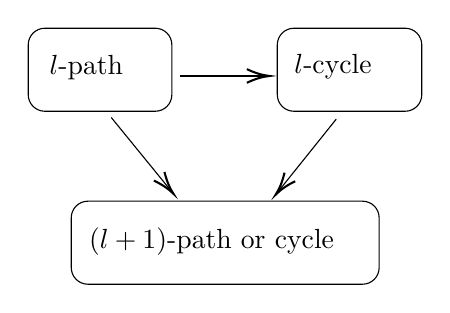
\begin{tikzpicture}[x=0.75pt,y=0.75pt,yscale=-1,xscale=1]
    % Rounded Rect [id:dp2247988663004169] 
    \draw   (100.6,84) .. controls (100.6,79.58) and (104.18,76) .. (108.6,76) -- (161.8,76) .. controls (166.22,76) and (169.8,79.58) .. (169.8,84) -- (169.8,108) .. controls (169.8,112.42) and (166.22,116) .. (161.8,116) -- (108.6,116) .. controls (104.18,116) and (100.6,112.42) .. (100.6,108) -- cycle ;
    % Rounded Rect [id:dp3322171879942837] 
    \draw   (220.6,84) .. controls (220.6,79.58) and (224.18,76) .. (228.6,76) -- (282.2,76) .. controls (286.62,76) and (290.2,79.58) .. (290.2,84) -- (290.2,108) .. controls (290.2,112.42) and (286.62,116) .. (282.2,116) -- (228.6,116) .. controls (224.18,116) and (220.6,112.42) .. (220.6,108) -- cycle ;
    % Rounded Rect [id:dp522325016929076] 
    \draw   (121.33,167.33) .. controls (121.33,162.92) and (124.92,159.33) .. (129.33,159.33) -- (261.67,159.33) .. controls (266.08,159.33) and (269.67,162.92) .. (269.67,167.33) -- (269.67,191.33) .. controls (269.67,195.75) and (266.08,199.33) .. (261.67,199.33) -- (129.33,199.33) .. controls (124.92,199.33) and (121.33,195.75) .. (121.33,191.33) -- cycle ;
    % Straight Lines [id:da4471732816066223] 
    \draw    (173.53,99) -- (214.87,99) ;
    \draw [shift={(216.87,99)}, rotate = 180] [color={rgb, 255:red, 0; green, 0; blue, 0 }  ][line width=0.75]    (10.93,-3.29) .. controls (6.95,-1.4) and (3.31,-0.3) .. (0,0) .. controls (3.31,0.3) and (6.95,1.4) .. (10.93,3.29)   ;
    % Straight Lines [id:da08077221270601986] 
    \draw    (140.6,119) -- (169.34,154.25) ;
    \draw [shift={(170.6,155.8)}, rotate = 230.81] [color={rgb, 255:red, 0; green, 0; blue, 0 }  ][line width=0.75]    (10.93,-3.29) .. controls (6.95,-1.4) and (3.31,-0.3) .. (0,0) .. controls (3.31,0.3) and (6.95,1.4) .. (10.93,3.29)   ;
    % Straight Lines [id:da17940502186011487] 
    \draw    (249,119.8) -- (221.05,154.64) ;
    \draw [shift={(219.8,156.2)}, rotate = 308.74] [color={rgb, 255:red, 0; green, 0; blue, 0 }  ][line width=0.75]    (10.93,-3.29) .. controls (6.95,-1.4) and (3.31,-0.3) .. (0,0) .. controls (3.31,0.3) and (6.95,1.4) .. (10.93,3.29)   ;

    % Text Nodes
    \draw (109.6,87.67) node [anchor=north west][inner sep=0.75pt]   [align=left] {$l$-path};
    \draw (227.6,87.27) node [anchor=north west][inner sep=0.75pt]   [align=left] {$l$-cycle};
    \draw (128.67,171) node [anchor=north west][inner sep=0.75pt]   [align=left] {$(l+1)$-path or cycle};
    \end{tikzpicture}
\end{center}

The algorithm considers two primary cases: when the object is a path and when it is a cycle. We will assume the algorithm is processing a graph with at
least $5$ vertices. The other cases were already covered by brute force.

\subsection{Path of Length $l$}

In this case, we start with a path \( P = \{x_1, e_1, \dots, x_{l}, e_{l}, x_{l + 1}\} \) of length \( l \). The goal is to find either a path of length \( l+1 \) or a cycle of length \( l \) or \( l+1 \). To assist in this process, we define the following variables:

\begin{itemize}
    \item \texttt{colors\_in\_path}: An array of size \( n \) where \texttt{colors\_in\_path[i]} is \texttt{True} if color \( i \) is used in the edges of the path.
    \item \texttt{vertices\_in\_path}: An array of size \( n \) where \texttt{vertices\_in\_path[i]} is \texttt{True} if vertex \( i \) is included in the path.
\end{itemize}

Let's divide the proof into two cases: when \( l \geq \left \lceil \frac{n}{2} \right \rceil \) and when \( l < \left \lceil \frac{n}{2} \right \rceil \).

\subsubsection{Case 1: \( l < \left \lceil \frac{n}{2} \right \rceil \)}

In this case, we select a color \( c \) that is not present among 
the edges of the current path. Since 
\( \deg(x_{l + 1}, c) \geq \left \lceil \frac{n}{2} \right \rceil \), 
and there are at most 
\( l < \left \lceil \frac{n}{2} \right \rceil \) 
vertices in the path, there must be a vertex 
\( y \) 
outside the path that is adjacent to 
\( x_{l + 1} \) via an edge in \( E(G_c) \). 
This guarantees that we can extend the path to a bigger path.

\begin{algorithm}[H]
    \caption{Path Extension for \( l < \left \lceil \frac{n}{2} \right \rceil \)}
    \begin{algorithmic}[1]
        \Function{Extend\_Path\_Small}{$G, P$}
        \State \textbf{assert} \( P.\text{size()} < \lceil \frac{n}{2} \rceil \)
        \State $last\_vertex \gets P.\text{back()}$
        \For{$color \in \{0, \dots, n-1\}$}
            \If{\textbf{not} $colors\_in\_path[color]$} \Comment{Search for an unused color}
                \For{$i \in \{0, \dots, n-1\}$}
                    \If{\textbf{not} $vertices\_in\_path[i]$} \Comment{Check vertices outside the path}
                        \State $edge \gets G.\text{check\_edge}(last\_vertex, i, color)$
                        \If{$edge \neq \text{None}$}
                            \State $vertices.\text{append}(i)$
                            \State $edges.\text{append}(edge)$
                            \State \Return Path($G$, $vertices$, $edges$) \Comment{Return extended path}
                        \EndIf
                    \EndIf
                \EndFor
            \EndIf
        \EndFor
        \State \textbf{assert False, "No valid extension found"}
    \EndFunction
    \end{algorithmic}
\end{algorithm}

The time complexity of this function is \( O(n) \). Since we 
only need to find a color that is not in the path’s colors 
,which takes \( O(n) \), and then locate a vertex outside 
the path that connects to the last vertex (also \( O(n) \)), 
the overall complexity remains linear in \( n \).

\subsubsection{Case 2: \( l \geq \left \lceil \frac{n}{2} \right \rceil \)}

First, remove the last edge and
vertex of the path and let $cx$ be a color that is not on the path and 
$cy$ be the color of the removed edge. We can check if the edge $\{x_1, x_{l}\}$ belongs to $G_{cx}$ or
to $G_{cy}$. If it does, we just found a cycle of size $l$. This can be done in $O(n)$ time complexity, the time need
to find a color outside the path and create the object Cycle. 


\begin{algorithm}[H]
    \caption{Part 1: Path Extension for \( l > \left \lceil \frac{n}{2} \right \rceil \)}
    \begin{algorithmic}
        \Function{Extend\_Path\_Big}{$G, P$}
            \State $cx \gets P.\text{edges}[-1].\text{color}$ \Comment{Color of the last edge in the path}
            \State $cy \gets \text{any color not in } colors\_in\_path$ \Comment{Find a color not in the path}
            \State $P.\text{pop\_back()}$ \Comment{Remove the last vertex from the path}
            \State $x \gets P.\text{vertices}[0]$ \Comment{First vertex in the path}
            \State $y \gets P.\text{vertices}[-1]$ \Comment{Last vertex in the updated path}

            \If{$edge \gets \text{check\_edge}(G, x, y, c) \neq \text{None}$}
                \State $vertices \gets P.\text{vertices.copy()}$
                \State $edges \gets P.\text{edges.copy()}$
                \State $edges.\text{append}(edge)$
                \State \Return Cycle($G$, $vertices$, $edges$) \Comment{Return cycle if found}
            \EndIf
        \EndFunction
    \end{algorithmic}
\end{algorithm}

We can now check if there exists a vertex $i$ outside the Path
such that $i$ is connects to the path on vertices $x_1$ and $x_l$
and uses colors $cx$ and $cy$, such as in the image below:

\begin{center}
    \tikzset{every picture/.style={line width=0.75pt}} %set default line width to 0.75pt        

    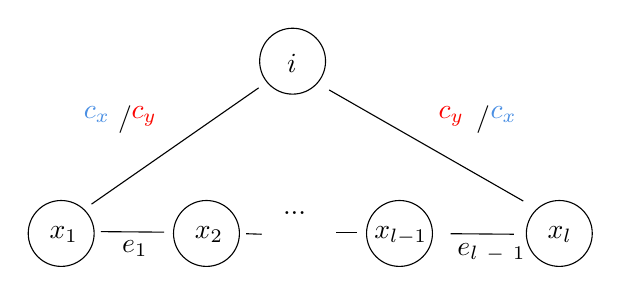
\begin{tikzpicture}[x=0.75pt,y=0.75pt,yscale=-1,xscale=1]
    %uncomment if require: \path (0,300); %set diagram left start at 0, and has height of 300
    
    %Shape: Circle [id:dp14076860311809425] 
    \draw  [color={rgb, 255:red, 0; green, 0; blue, 0 }  ,draw opacity=1 ] (100,135.88) .. controls (100,127.11) and (107.11,120) .. (115.88,120) .. controls (124.64,120) and (131.75,127.11) .. (131.75,135.88) .. controls (131.75,144.64) and (124.64,151.75) .. (115.88,151.75) .. controls (107.11,151.75) and (100,144.64) .. (100,135.88) -- cycle ;
    %Shape: Circle [id:dp9718918515389369] 
    \draw  [color={rgb, 255:red, 0; green, 0; blue, 0 }  ,draw opacity=1 ] (340,135.88) .. controls (340,127.11) and (347.11,120) .. (355.88,120) .. controls (364.64,120) and (371.75,127.11) .. (371.75,135.88) .. controls (371.75,144.64) and (364.64,151.75) .. (355.88,151.75) .. controls (347.11,151.75) and (340,144.64) .. (340,135.88) -- cycle ;
    %Shape: Circle [id:dp22152249244642985] 
    \draw  [color={rgb, 255:red, 0; green, 0; blue, 0 }  ,draw opacity=1 ] (170,135.88) .. controls (170,127.11) and (177.11,120) .. (185.88,120) .. controls (194.64,120) and (201.75,127.11) .. (201.75,135.88) .. controls (201.75,144.64) and (194.64,151.75) .. (185.88,151.75) .. controls (177.11,151.75) and (170,144.64) .. (170,135.88) -- cycle ;
    %Straight Lines [id:da5129055940889523] 
    \draw    (135,135) -- (165.5,135.25) ;
    %Straight Lines [id:da581278780757175] 
    \draw    (303.5,136) -- (334,136.25) ;
    %Shape: Circle [id:dp2164326053488742] 
    \draw  [color={rgb, 255:red, 0; green, 0; blue, 0 }  ,draw opacity=1 ] (263,135.88) .. controls (263,127.11) and (270.11,120) .. (278.88,120) .. controls (287.64,120) and (294.75,127.11) .. (294.75,135.88) .. controls (294.75,144.64) and (287.64,151.75) .. (278.88,151.75) .. controls (270.11,151.75) and (263,144.64) .. (263,135.88) -- cycle ;
    %Straight Lines [id:da9291156181154486] 
    \draw    (248.5,135.25) -- (258.5,135.25) ;
    %Straight Lines [id:da2577772310594443] 
    \draw    (205,136) -- (212.5,136.25) ;
    %Shape: Circle [id:dp2553341740528331] 
    \draw  [color={rgb, 255:red, 0; green, 0; blue, 0 }  ,draw opacity=1 ] (211.5,52.88) .. controls (211.5,44.11) and (218.61,37) .. (227.38,37) .. controls (236.14,37) and (243.25,44.11) .. (243.25,52.88) .. controls (243.25,61.64) and (236.14,68.75) .. (227.38,68.75) .. controls (218.61,68.75) and (211.5,61.64) .. (211.5,52.88) -- cycle ;
    %Straight Lines [id:da500585581947927] 
    \draw    (130.5,121.75) -- (211,65.75) ;
    %Straight Lines [id:da13872883018767035] 
    \draw    (338.5,120.25) -- (245,66.75) ;
    
    % Text Node
    \draw (109,131.4) node [anchor=north west][inner sep=0.75pt]    {$x_{1}$};
    % Text Node
    \draw (349,131.4) node [anchor=north west][inner sep=0.75pt]    {$x_{l}$};
    % Text Node
    \draw (179,131.4) node [anchor=north west][inner sep=0.75pt]    {$x_{2}$};
    % Text Node
    \draw (265.5,131.4) node [anchor=north west][inner sep=0.75pt]    {$x_{l-1}$};
    % Text Node
    \draw (221.5,124) node [anchor=north west][inner sep=0.75pt]   [align=left] {...};
    % Text Node
    \draw (144,137.9) node [anchor=north west][inner sep=0.75pt]    {$e_{1}$};
    % Text Node
    \draw (305.5,139.4) node [anchor=north west][inner sep=0.75pt]    {$e_{l\ -\ 1}$};
    % Text Node
    \draw (223.5,48.4) node [anchor=north west][inner sep=0.75pt]    {$i$};
    % Text Node
    \draw (125.5,73.4) node [anchor=north west][inner sep=0.75pt]    {$\textcolor[rgb]{0.29,0.56,0.89}{c_{x}}$};
    % Text Node
    \draw (321.5,73.4) node [anchor=north west][inner sep=0.75pt]    {$\textcolor[rgb]{0.29,0.56,0.89}{c}\textcolor[rgb]{0.29,0.56,0.89}{_{x}}$};
    % Text Node
    \draw (148.5,73.4) node [anchor=north west][inner sep=0.75pt]    {$\textcolor[rgb]{0.99,0.01,0.01}{c_{\textcolor[rgb]{0.98,0.03,0}{y}}}$};
    % Text Node
    \draw (142,73) node [anchor=north west][inner sep=0.75pt]   [align=left] {/};
    % Text Node
    \draw (296.5,73.4) node [anchor=north west][inner sep=0.75pt]    {$\textcolor[rgb]{0.99,0.01,0.01}{c}\textcolor[rgb]{0.99,0.01,0.01}{_{\textcolor[rgb]{0.98,0.03,0}{y}}}$};
    % Text Node
    \draw (314.5,73) node [anchor=north west][inner sep=0.75pt]   [align=left] {/};
    
    
    \end{tikzpicture}
    
\end{center}

This part can also be done on $O(n)$ time complexity with
the code below:

\begin{algorithm}[H]
    \caption{Part 3: Path Extension for \( l > \left \lceil \frac{n}{2} \right \rceil \)}
    \begin{algorithmic}
        \Function{Extend\_Path\_Big}{$G, P$}
            \For{$[c1, c2] \in [[cx, cy], [cy, cx]]$} \Comment{Try both color pairs}
                \For{$i \in \{0, \dots, n-1\}$}
                    \If{\textbf{not} $vertices\_in\_path[i]$} \Comment{Check vertices outside the path}
                        \State $edgeX \gets \text{check\_edge}(G, x, i, c1)$
                        \State $edgeY \gets \text{check\_edge}(G, y, i, c2)$
                        \If{$(edgeX \neq \text{None})$ and $(edgeY \neq \text{None})$}
                            \State $vertices \gets P.\text{vertices.copy()}$
                            \State $vertices.\text{append}(i)$
                            \State $edges \gets P.\text{edges.copy()}$
                            \State $edges.\text{append}(edgeY)$
                            \State $edges.\text{append}(edgeX)$
                            \State \Return Cycle($G$, $vertices$, $edges$) \Comment{Return cycle if found}
                        \EndIf
                    \EndIf
                \EndFor
            \EndFor

            \State \textbf{assert False, "No valid extension found"}
        \EndFunction
    \end{algorithmic}
\end{algorithm}

Let's define $I_1 = \{i \in [l - 2]: \{x_1, x_{i + 1}\} \in E_{G_cx}\}$ and 
$I_2 = \{i \in [2, l - 1]: \{x_i, x_{l}\} \in E_{G_cy}\}$.

Note that as we did not find a cycle yet, 

$$
|N_{G_{c_x}}(x_1) \backslash V(P)| + |N_{G_{c_y}}(x_l) \backslash V(P)| \leq n - l,
$$

otherwise, by Dirichlet Principle, we would have found a cycle
with the procedures above. Thus, we have that

$$
|I_1| + |I_2| \geq \frac{n}{2} + \frac{n}{2} - |N_{G_cx}(x_1) \backslash V(P)| - |N_{G_cy}(x_l) \backslash V(P)| \geq l.
$$

As we $I_1$ and $I_2$ share the same set of vertices of size
$l - 2$, $I_1 \cap I_2 \neq \emptyset$. Given an element
$i \in I_1 \cap I_2$, we can build a cycle with size $l$ with
the following crossing, removing edge $x_i$.

\begin{center}
\tikzset{every picture/.style={line width=0.75pt}} %set default line width to 0.75pt        

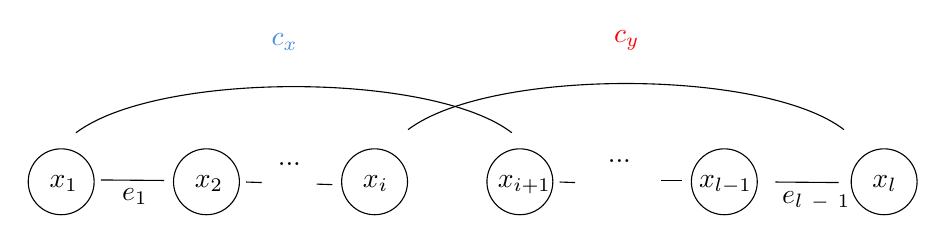
\begin{tikzpicture}[x=0.75pt,y=0.75pt,yscale=-1,xscale=1]
%uncomment if require: \path (0,300); %set diagram left start at 0, and has height of 300

%Shape: Circle [id:dp14076860311809425] 
\draw  [color={rgb, 255:red, 0; green, 0; blue, 0 }  ,draw opacity=1 ] (100,135.88) .. controls (100,127.11) and (107.11,120) .. (115.88,120) .. controls (124.64,120) and (131.75,127.11) .. (131.75,135.88) .. controls (131.75,144.64) and (124.64,151.75) .. (115.88,151.75) .. controls (107.11,151.75) and (100,144.64) .. (100,135.88) -- cycle ;
%Shape: Circle [id:dp9718918515389369] 
\draw  [color={rgb, 255:red, 0; green, 0; blue, 0 }  ,draw opacity=1 ] (496.5,135.88) .. controls (496.5,127.11) and (503.61,120) .. (512.38,120) .. controls (521.14,120) and (528.25,127.11) .. (528.25,135.88) .. controls (528.25,144.64) and (521.14,151.75) .. (512.38,151.75) .. controls (503.61,151.75) and (496.5,144.64) .. (496.5,135.88) -- cycle ;
%Shape: Circle [id:dp22152249244642985] 
\draw  [color={rgb, 255:red, 0; green, 0; blue, 0 }  ,draw opacity=1 ] (170,135.88) .. controls (170,127.11) and (177.11,120) .. (185.88,120) .. controls (194.64,120) and (201.75,127.11) .. (201.75,135.88) .. controls (201.75,144.64) and (194.64,151.75) .. (185.88,151.75) .. controls (177.11,151.75) and (170,144.64) .. (170,135.88) -- cycle ;
%Straight Lines [id:da5129055940889523] 
\draw    (135,135) -- (165.5,135.25) ;
%Straight Lines [id:da581278780757175] 
\draw    (460,136) -- (490.5,136.25) ;
%Shape: Circle [id:dp2164326053488742] 
\draw  [color={rgb, 255:red, 0; green, 0; blue, 0 }  ,draw opacity=1 ] (419.5,135.88) .. controls (419.5,127.11) and (426.61,120) .. (435.38,120) .. controls (444.14,120) and (451.25,127.11) .. (451.25,135.88) .. controls (451.25,144.64) and (444.14,151.75) .. (435.38,151.75) .. controls (426.61,151.75) and (419.5,144.64) .. (419.5,135.88) -- cycle ;
%Straight Lines [id:da9291156181154486] 
\draw    (405,135.25) -- (415,135.25) ;
%Straight Lines [id:da2577772310594443] 
\draw    (205,136) -- (212.5,136.25) ;
%Shape: Circle [id:dp8825188362565558] 
\draw  [color={rgb, 255:red, 0; green, 0; blue, 0 }  ,draw opacity=1 ] (251,135.88) .. controls (251,127.11) and (258.11,120) .. (266.88,120) .. controls (275.64,120) and (282.75,127.11) .. (282.75,135.88) .. controls (282.75,144.64) and (275.64,151.75) .. (266.88,151.75) .. controls (258.11,151.75) and (251,144.64) .. (251,135.88) -- cycle ;
%Shape: Circle [id:dp9134750344031234] 
\draw  [color={rgb, 255:red, 0; green, 0; blue, 0 }  ,draw opacity=1 ] (321,135.88) .. controls (321,127.11) and (328.11,120) .. (336.88,120) .. controls (345.64,120) and (352.75,127.11) .. (352.75,135.88) .. controls (352.75,144.64) and (345.64,151.75) .. (336.88,151.75) .. controls (328.11,151.75) and (321,144.64) .. (321,135.88) -- cycle ;
%Straight Lines [id:da6587077764610608] 
\draw    (356,136) -- (363.5,136.25) ;
%Straight Lines [id:da08873759090043654] 
\draw    (239,137) -- (246.5,137.25) ;
%Curve Lines [id:da934768158738368] 
\draw    (123,112.25) .. controls (163,82.25) and (295,83) .. (333,112.25) ;
%Curve Lines [id:da06750067448598662] 
\draw    (283,110.75) .. controls (323,80.75) and (455,81.5) .. (493,110.75) ;

% Text Node
\draw (109,131.4) node [anchor=north west][inner sep=0.75pt]    {$x_{1}$};
% Text Node
\draw (505.5,131.4) node [anchor=north west][inner sep=0.75pt]    {$x_{l}$};
% Text Node
\draw (179,131.4) node [anchor=north west][inner sep=0.75pt]    {$x_{2}$};
% Text Node
\draw (422,131.4) node [anchor=north west][inner sep=0.75pt]    {$x_{l-1}$};
% Text Node
\draw (378,124) node [anchor=north west][inner sep=0.75pt]   [align=left] {...};
% Text Node
\draw (144,137.9) node [anchor=north west][inner sep=0.75pt]    {$e_{1}$};
% Text Node
\draw (462,139.4) node [anchor=north west][inner sep=0.75pt]    {$e_{l\ -\ 1}$};
% Text Node
\draw (216,63.4) node [anchor=north west][inner sep=0.75pt]    {$\textcolor[rgb]{0.29,0.56,0.89}{c_{x}}$};
% Text Node
\draw (381,61.9) node [anchor=north west][inner sep=0.75pt]    {$\textcolor[rgb]{0.99,0.01,0.01}{c_{\textcolor[rgb]{0.98,0.03,0}{y}}}$};
% Text Node
\draw (219,125.5) node [anchor=north west][inner sep=0.75pt]   [align=left] {...};
% Text Node
\draw (260,131.4) node [anchor=north west][inner sep=0.75pt]    {$x_{i}$};
% Text Node
\draw (325,131.4) node [anchor=north west][inner sep=0.75pt]    {$x_{i+1}$};


\end{tikzpicture}

\end{center}

Then, for this case, we just need to find an intersection
for $I_1$ and $I_2$ and build the solution. This can also
be done in $O(n)$ with the code below:

\begin{algorithm}[H]
    \caption{Part 3: Path Extension for \( l > \left \lceil \frac{n}{2} \right \rceil \)}
    \begin{algorithmic}[1]
        \Function{Extend\_Path\_Big}{$G, P$}
            \For{$i \gets 1$ to $|P.\text{vertices}| - 2$}
                \State $u \gets P.\text{vertices}[i]$
                \State $v \gets P.\text{vertices}[i + 1]$
                \State $edgeX \gets \text{check\_edge}(G, x, v, cx)$
                \State $edgeY \gets G.\text{check\_edge}(G, u, y, cy)$

                \If{$(edgeX \neq \text{None})$ and $(edgeY \neq \text{None})$} 
                    \State $vertices \gets P.\text{vertices}[1:i] + [y] + \text{Reverse}(P.\text{vertices}[i + 1:l])$
                    \State $edges \gets P.\text{edges}[1:i - 1] + [edgeY]$

                    \For{$j \gets |P.\text{vertices}| - 1$ down to $i + 1$}
                        \State $vertices.\text{append}(P.\text{vertices}[j - 1])$
                        \State $edges.\text{append}(P.\text{edges}[j - 1])$
                    \EndFor
                    \State $edges.\text{append}(edgeX)$ \Comment{Add $edgeX$ to close the cycle}
                    \State \Return Cycle($G$, $vertices$, $edges$)
                \EndIf
            \EndFor
            \State \Return \text{None} \Comment{Return None if no cycle found}
        \EndFunction
    \end{algorithmic}
\end{algorithm}


\subsection{Cycle of length $l$}

In this case, we start with a cycle \( C = \{x_1, e_1, \dots, x_{l}, e_{l}, x_{l+1} = x_{1}\} \) of length \( l \). 
The goal is to find either a path of length \( l+1 \) or a cycle of length \( l \) or \( l+1 \). 
To assist in this process, we define the following variables:

\begin{itemize}
    \item \texttt{colors\_in\_cycle}: An array of size \( n \) where \texttt{colors\_in\_cycle[i]} is \texttt{True} if color \( i \) is used in the edges of the cycle.
    \item \texttt{vertices\_in\_cycle}: An array of size \( n \) where \texttt{vertices\_in\_cycle[i]} is \texttt{True} if vertex \( i \) is included in the cycle.
\end{itemize}

These variables can be calculated in \( O(n) \) time complexity. We may assume the cycle is of length at least \( \left \lceil \frac{n}{2} \right \rceil \).
Let's divide the proof into two cases: when \( l < n - 1 \) and when \( l = n - 1 \).

\subsection{Case 1: $n - 1 \neq \ell \geq \left \lceil \frac{n}{2} \right \rceil + 1$}

Let $c_1$ and $c_2$ be two colors that are not in the cycle. We will try to find
two vertices that are both $u$ and $v$ outside the cycle and the edge $\{u, v\}$ is in $G_{c_i}$, $i$ being $1$ or $2$.
If such vertices exist, there is also an edge $\{u, x_i\} \in G_{c_{3-i}}$, because

$$
l + |N_{G_{c_{3-i}}}(u)| \geq 2 \left\lceil \frac{n}{2} \right\rceil + 1 \geq n + 1.
$$

Taking $x_j$ as a vertex on the cycle such that $\{x_j, u\} \in G_{c_{3-i}}$, we can build a 
path of length $l + 1$ by removing the edge $\{x_j, x_{j + 1}\}$ and adding the edges $edge(u, v, c_i)$ and 
$edge(u, x_j, c_{3-i})$, as shown in the diagram below:

\begin{center}

\tikzset{every picture/.style={line width=0.75pt}} %set default line width to 0.75pt        

\begin{tikzpicture}[x=0.75pt,y=0.75pt,yscale=-1,xscale=1]
%uncomment if require: \path (0,300); %set diagram left start at 0, and has height of 300

%Shape: Circle [id:dp17546919027444852] 
\draw   (300,32.91) .. controls (300,25.78) and (305.78,20) .. (312.91,20) .. controls (320.03,20) and (325.81,25.78) .. (325.81,32.91) .. controls (325.81,40.03) and (320.03,45.81) .. (312.91,45.81) .. controls (305.78,45.81) and (300,40.03) .. (300,32.91) -- cycle ;
%Shape: Circle [id:dp6772890116560196] 
\draw   (260,162.91) .. controls (260,155.78) and (265.78,150) .. (272.91,150) .. controls (280.03,150) and (285.81,155.78) .. (285.81,162.91) .. controls (285.81,170.03) and (280.03,175.81) .. (272.91,175.81) .. controls (265.78,175.81) and (260,170.03) .. (260,162.91) -- cycle ;
%Shape: Circle [id:dp5871526391848064] 
\draw   (340,162.91) .. controls (340,155.78) and (345.78,150) .. (352.91,150) .. controls (360.03,150) and (365.81,155.78) .. (365.81,162.91) .. controls (365.81,170.03) and (360.03,175.81) .. (352.91,175.81) .. controls (345.78,175.81) and (340,170.03) .. (340,162.91) -- cycle ;
%Shape: Circle [id:dp07729495910565454] 
\draw   (390,212.91) .. controls (390,205.78) and (395.78,200) .. (402.91,200) .. controls (410.03,200) and (415.81,205.78) .. (415.81,212.91) .. controls (415.81,220.03) and (410.03,225.81) .. (402.91,225.81) .. controls (395.78,225.81) and (390,220.03) .. (390,212.91) -- cycle ;
%Shape: Circle [id:dp262131491828823] 
\draw   (210,212.91) .. controls (210,205.78) and (215.78,200) .. (222.91,200) .. controls (230.03,200) and (235.81,205.78) .. (235.81,212.91) .. controls (235.81,220.03) and (230.03,225.81) .. (222.91,225.81) .. controls (215.78,225.81) and (210,220.03) .. (210,212.91) -- cycle ;
%Straight Lines [id:da3647606509042579] 
\draw    (290.33,164.05) -- (311,164.05) -- (335.67,164.05) ;
%Straight Lines [id:da10861800407645683] 
\draw    (238.33,199.38) -- (261,176.05) ;
%Straight Lines [id:da2699490633303564] 
\draw    (391,199.38) -- (367.67,176.05) ;
%Straight Lines [id:da35645617170084576] 
\draw    (235,226.72) -- (277.67,254.72) ;
%Straight Lines [id:da36572819250411115] 
\draw    (388.33,227.38) -- (347.67,254.05) ;
%Shape: Circle [id:dp5515582428891825] 
\draw   (300,92.91) .. controls (300,85.78) and (305.78,80) .. (312.91,80) .. controls (320.03,80) and (325.81,85.78) .. (325.81,92.91) .. controls (325.81,100.03) and (320.03,105.81) .. (312.91,105.81) .. controls (305.78,105.81) and (300,100.03) .. (300,92.91) -- cycle ;
%Straight Lines [id:da6018921647481235] 
\draw [color={rgb, 255:red, 74; green, 144; blue, 226 }  ,draw opacity=1 ]   (313,50.05) -- (313,76.05) ;
%Curve Lines [id:da9530976173140503] 
\draw [color={rgb, 255:red, 208; green, 2; blue, 27 }  ,draw opacity=1 ]   (337,97.38) .. controls (377.67,90.72) and (545,248.72) .. (373,264.72) ;

% Text Node
\draw (345,157.4) node [anchor=north west][inner sep=0.75pt]    {$x_{1}$};
% Text Node
\draw (265,157.4) node [anchor=north west][inner sep=0.75pt]    {$x_{l}$};
% Text Node
\draw (306,27.4) node [anchor=north west][inner sep=0.75pt]    {$v$};
% Text Node
\draw (395,207.4) node [anchor=north west][inner sep=0.75pt]    {$x_{2}$};
% Text Node
\draw (215,207.4) node [anchor=north west][inner sep=0.75pt]    {$x_{l}$};
% Text Node
\draw (305.33,143.73) node [anchor=north west][inner sep=0.75pt]    {$e_{l}$};
% Text Node
\draw (228,169.4) node [anchor=north west][inner sep=0.75pt]    {$e_{l}{}_{-1}$};
% Text Node
\draw (382.67,173.4) node [anchor=north west][inner sep=0.75pt]    {$e_{1}{}$};
% Text Node
\draw (306,242) node [anchor=north west][inner sep=0.75pt]   [align=left] {...};
% Text Node
\draw (306,87.4) node [anchor=north west][inner sep=0.75pt]    {$u$};
% Text Node
\draw (320.67,53.07) node [anchor=north west][inner sep=0.75pt]  [font=\normalsize,color={rgb, 255:red, 74; green, 144; blue, 226 }  ,opacity=1 ]  {$c_{i}$};
% Text Node
\draw (427.33,125.73) node [anchor=north west][inner sep=0.75pt]  [font=\normalsize,color={rgb, 255:red, 208; green, 2; blue, 27 }  ,opacity=1 ]  {$c_{3-i}$};

\end{tikzpicture}

\end{center}

This can be done in $O(n^2)$ time complexity with the code below:

\begin{algorithm}[H]
    \caption{Part 1: Cycle Extension for \( l < n - 1 \)}
    \begin{algorithmic}
        \Function{Extend\_Cycle}{$G, P$}
            \For{$[ci, cj] \in [[c1, c2], [c2, c1]]$} \Comment{Try both color pairs}
                \For{$u \in \{0, \dots, n-1\}$}
                    \For{$v \in \{0, \dots, n-1\}$}
                        \If{\textbf{not} $vertices\_in\_cycle[u]$ \text{and} \\
                            \hspace{7em}\textbf{not} $vertices\_in\_cycle[v]$}
                            \Comment{Check vertices are outside the cycle}
                            \State $edgeV \gets \text{check\_edge}(G, u, v, ci)$
                            \State $edgeW \gets \text{check\_edge}(G, u, w, cj)$
                            \If{$(edgeU \neq \text{None})$ and $(edgeV \neq \text{None})$}
                                \For{$w \in G.adjacency[j][v]$}
                                    \If{\textbf{not} $vertices\_in\_cycle[w]$}
                                        \State \textbf{continue}
                                    \EndIf
                                    \Comment{Anexa o caminho $uvw$ ao ciclo}
                                    \State $w\_id \gets C.vertices.\text{index}(w)$
                                    \State $vertices \gets C.vertices[w\_id + 1:] +$
                                    \State \hspace{2.5em} $C.vertices[:w\_id + 1] +$
                                    \State \hspace{2.5em} $[u, v]$
                                    \State $edge \gets C.edges[w\_id + 1:] +$
                                    \State \hspace{2.5em} $C.edges[:w\_id] +$
                                    \State \hspace{2.5em} $[edgeW, edgeV]$
                                    \State
                                    \Return $\text{Path}(G, vertices, edges)$
                                \EndFor
                                \State \textbf{assert False, "Should not reach here"}
                            \EndIf
                        \EndIf
                    \EndFor
                \EndFor
            \EndFor
            \State \textbf{...}
        \EndFunction
    \end{algorithmic}
\end{algorithm}

The complexity is in fact $O(n^2)$ because once we find valid edges $edgeV$ and $edgeW$,
it is guaranteed that we will find a vertex $w$ that is in the cycle.

From now on, for every vertex $u$ outside the cycle, every edge of colors $c_1$ and $c_2$ incident to 
$u$ must also be incident to the cycle. 
Take $u \in V \backslash V(C)$. Let 

$$
I_1 \coloneqq \{i \in [l]: edge(u, x_{i + 1}, c_1) \in E_G\} \text{ and } I_2 \coloneqq \{i \in [l]: edge(x_i, u, c_2) \in E_G\},
$$

where $x_{l + 1} = x_1$. We have that $|I_1| + |I_2| = |N_{G_{c_1}}(u)| + |N_{G_{c_2}}(u)| \geq n > l$. Thus, 
from Dirichlet Principle, $I_1 \cap I_2 \neq \emptyset$. In this case, we can build a cycle of length $l + 1$
with the following crossing, removing the edge $x_i$:
\begin{center}
\tikzset{every picture/.style={line width=0.75pt}} %set default line width to 0.75pt        

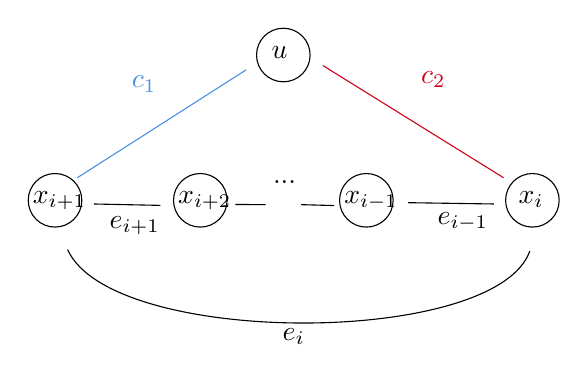
\begin{tikzpicture}[x=0.75pt,y=0.75pt,yscale=-1,xscale=1]
%uncomment if require: \path (0,300); %set diagram left start at 0, and has height of 300

%Shape: Circle [id:dp6772890116560196] 
\draw   (260,162.91) .. controls (260,155.78) and (265.78,150) .. (272.91,150) .. controls (280.03,150) and (285.81,155.78) .. (285.81,162.91) .. controls (285.81,170.03) and (280.03,175.81) .. (272.91,175.81) .. controls (265.78,175.81) and (260,170.03) .. (260,162.91) -- cycle ;
%Shape: Circle [id:dp5871526391848064] 
\draw   (340,162.91) .. controls (340,155.78) and (345.78,150) .. (352.91,150) .. controls (360.03,150) and (365.81,155.78) .. (365.81,162.91) .. controls (365.81,170.03) and (360.03,175.81) .. (352.91,175.81) .. controls (345.78,175.81) and (340,170.03) .. (340,162.91) -- cycle ;
%Shape: Circle [id:dp07729495910565454] 
\draw   (420,162.91) .. controls (420,155.78) and (425.78,150) .. (432.91,150) .. controls (440.03,150) and (445.81,155.78) .. (445.81,162.91) .. controls (445.81,170.03) and (440.03,175.81) .. (432.91,175.81) .. controls (425.78,175.81) and (420,170.03) .. (420,162.91) -- cycle ;
%Shape: Circle [id:dp262131491828823] 
\draw   (190,162.91) .. controls (190,155.78) and (195.78,150) .. (202.91,150) .. controls (210.03,150) and (215.81,155.78) .. (215.81,162.91) .. controls (215.81,170.03) and (210.03,175.81) .. (202.91,175.81) .. controls (195.78,175.81) and (190,170.03) .. (190,162.91) -- cycle ;
%Straight Lines [id:da10861800407645683] 
\draw    (221.67,164.68) -- (253.67,165.35) ;
%Straight Lines [id:da2699490633303564] 
\draw    (414.33,164.68) -- (373,164.05) ;
%Shape: Circle [id:dp5515582428891825] 
\draw   (300,92.91) .. controls (300,85.78) and (305.78,80) .. (312.91,80) .. controls (320.03,80) and (325.81,85.78) .. (325.81,92.91) .. controls (325.81,100.03) and (320.03,105.81) .. (312.91,105.81) .. controls (305.78,105.81) and (300,100.03) .. (300,92.91) -- cycle ;
%Straight Lines [id:da6018921647481235] 
\draw [color={rgb, 255:red, 74; green, 144; blue, 226 }  ,draw opacity=1 ]   (213.67,152.02) -- (295,100.05) ;
%Straight Lines [id:da536121074656983] 
\draw    (289.81,164.91) -- (304.33,165) ;
%Straight Lines [id:da7967913679803297] 
\draw    (321.48,165) -- (337.33,165.44) ;
%Straight Lines [id:da2711467439601347] 
\draw [color={rgb, 255:red, 208; green, 2; blue, 27 }  ,draw opacity=1 ]   (332,98) -- (419,152.02) ;
%Curve Lines [id:da25468149628094827] 
\draw    (209,186.68) .. controls (230,233.7) and (415.33,233.7) .. (431.67,187.35) ;

% Text Node
\draw (341,157.4) node [anchor=north west][inner sep=0.75pt]    {$x_{i-1}$};
% Text Node
\draw (261,157.4) node [anchor=north west][inner sep=0.75pt]    {$x_{i+2}$};
% Text Node
\draw (425,157.4) node [anchor=north west][inner sep=0.75pt]    {$x_{i}$};
% Text Node
\draw (191,157.4) node [anchor=north west][inner sep=0.75pt]    {$x_{i+1}$};
% Text Node
\draw (228,169.4) node [anchor=north west][inner sep=0.75pt]    {$e_{i+1}{}$};
% Text Node
\draw (386,167.4) node [anchor=north west][inner sep=0.75pt]    {$e_{i-1}{}$};
% Text Node
\draw (306.67,152) node [anchor=north west][inner sep=0.75pt]   [align=left] {...};
% Text Node
\draw (306,87.4) node [anchor=north west][inner sep=0.75pt]    {$u$};
% Text Node
\draw (238.67,101.73) node [anchor=north west][inner sep=0.75pt]  [font=\normalsize,color={rgb, 255:red, 74; green, 144; blue, 226 }  ,opacity=1 ]  {$c_{1}$};
% Text Node
\draw (378,99.73) node [anchor=north west][inner sep=0.75pt]  [font=\normalsize,color={rgb, 255:red, 208; green, 2; blue, 27 }  ,opacity=1 ]  {$c_{2}$};
% Text Node
\draw (311.33,223.4) node [anchor=north west][inner sep=0.75pt]    {$e_{i}{}$};


\end{tikzpicture}
\end{center}


The code for finding this crossing is shown below:

\begin{algorithm}[H]
    \caption{Part 2: Cycle Extension for \( l < n - 1 \)}
    \begin{algorithmic}
        \Function{Extend\_Cycle}{$G, C$}
            \For{$u \in \{0, \dots, n-1\}$}
                \If{\textbf{not} $vertices\_in\_cycle[u]$}
                    \For{$i \in \{0, \dots, |C.vertices| - 1\}$}
                        \State $xi \gets vertices[i]$
                        \State $xj \gets vertices[(i + 1) \bmod |vertices|]$

                        \State $edge1 \gets \text{check\_edge}(G, u, xj, c1)$
                        \State $edge2 \gets \text{check\_edge}(G, u, xi, c2)$
                        
                        \If{$edge1 \neq \text{None} \land edge2 \neq \text{None}$}
                            \State $vertices \gets C.vertices[i + 1:] \hspace{0.3em} +$
                            \State \hspace{2.5em} $C.vertices[:i + 1] + [u]$

                            \State $edges \gets edges[i + 1:] \hspace{0.3em} +$
                            \State \hspace{2.5em} $edges[:i] \hspace{0.3em} +$
                            \State \hspace{2.5em} $[edge1, edge2]$
                            \State \Return $\text{Cycle}(G, vertices, edges)$
                        \EndIf
                    \EndFor
                \EndIf
            \EndFor
            \State \textbf{assert False, "Should not reach here"}
        \EndFunction
    \end{algorithmic}
\end{algorithm}

This part works in $O(n)$ time complexity, as we as soon as we find a vertex outside the cycle,
we just make a linear search for a crossing and find the solution.

\subsection{Case 2: Cycle of length $l = n - 1$}

\subsubsection{Auxiliary Functions}

\begin{itemize}
    \item \texttt{find\_adjacency(u, color, vertex\_positions)}: This function gives the indexes of the 
    vertices that are adjacent to $u$ with color $color$, based on the current 
    positions of the vertices. This is useful when we need to change the vertex position in the cycle.
    The algorithm is shown below:

    \begin{algorithm}
        \caption{Find Adjacency Index List for a Given Source and Color}
        \begin{algorithmic}[1]
            \Function{Find\_Adjacency}{$u, color, vertex\_positions$}
                \State $ans \gets []$
                \For{$tgt \in G.\text{adjacency}[color][u]$}
                    \State $ans.\text{append}(vertex\_positions[tgt])$
                \EndFor
                \State \Return $ans$ \Comment{Return the list of positions}
            \EndFunction
        \end{algorithmic}
    \end{algorithm}

    It's complexity is $O(n)$, as we just need to iterate over the adjacency list of $u$ with color $color$.

    \item \texttt{find\_answer(G, y, cy, C, i)}: Let $G$ be the graph, $C$ a cycle with
    size $n-1$, $y$ be the only vertex outside the cycle, $c_y$ be the only color
    outside the cycle and $i$ the index of the edge $e_i$ to be removed. This function 
    builds a cycle with size $n$ by removing the edge $e_i$ and adding the edges
    $edge(x_{i}, y, e_i.color)$ and $edge(y, x_{i+1}, c_y)$.

    The algorithm is shown below:

    \begin{algorithm}
        \caption{Find Answer for \( l = n - 1 \)}
        \begin{algorithmic}[1]
            \Function{Find\_Answer}{$G, y, cy, C, i$}
                \State $vertices \gets C.vertices[i + 1:] + C.vertices[:i + 1] + [y]$
                \State $edges \gets C.edges[i + 1:] + C.edges[:i]$
                \State \hspace{2.5em} $+ [G.\text{get\_edge}(vertices[-1], y, C.edges[i].color), G.\text{get\_edge}(y, C.vertices[0], cy)]$
                \State \Return $\text{Cycle}(G, vertices, edges)$
            \EndFunction
        \end{algorithmic}
    \end{algorithm}

    The complexity is $O(n)$, as we just need to rotate some lists of size $n$ and the other operations are $O(1)$.
\end{itemize}

\subsubsection{Algorithm}

This case is a bit more complicated. It is always the last iteration of the algorithm and will
find the desired cycle.

Let $y$ and $cy$ be the vertex and color that are not in the cycle. We will rearrange the labels
of the colors such that the remaining color has label $n - 1$. Let's also define the following variables:

\begin{itemize}
    \item \texttt{new\_color\_id}: An array of size \( n \) where \texttt{new\_color\_id[i]} is the new label of color \( i \),
    \item \texttt{vertex\_position\_on\_cycle}: An array of size \( n \) where \texttt{vertex\_position\_on\_cycle[i]} is the position of vertex \( i \) in the cycle.
    \item \texttt{color\_in\_position}: An array of size \( n \) where \texttt{color\_in\_position[i]} is the color of the edge that connects the vertices \( i \) and \( i + 1 \) in the cycle.
\end{itemize}

These variables can be calculated in \( O(n) \) time complexity. The algorithm is shown below:

\begin{algorithm}
    \caption{Part 1: Cycle Extension for \( l = n - 1 \)}
    \begin{algorithmic}
        \Function{Extend\_Cycle}{$G, C$}
            \State $new\_color\_id \gets [-1] \times n$
            \State $y \gets \text{first } i \in \{0, \dots, n-1\} \text{ such that } \textbf{not } vertices\_in\_cycle[i]$
            \State $cy \gets \text{first } i \in \{0, \dots, n-1\} \text{ such that } \textbf{not } colors\_in\_cycle[i]$
            \State $new\_color\_id[cy] \gets n - 1$
            
            \For{$i \in \{0, \dots, C.size() - 1\}$}
                \State $new\_color\_id[color] \gets i$
                \State $color\_in\_position \gets C.edges[i].color$
            \EndFor
            
            \State $vertex\_position\_on\_cycle \gets [-1] \times n$
            \For{$i \in \{0, \dots, C.size() - 1\}$}
                \State $vertex\_position\_on\_cycle[cycle.vertices[i]] \gets i$
            \EndFor
        \EndFunction
    \end{algorithmic}
\end{algorithm}

Let's build the following digraph on the same vertex set of $G$. There is a visual representation
of the digraph below:

$$
A(D) = \bigcup_{i \in \{0,..., n - 2\}} \{\{x_i, z\} : z \neq x_{i + 1}, edge(x_i, z, C.edge[i].color) \in E(G)\}.
$$

\begin{center}


\tikzset{every picture/.style={line width=0.75pt}} %set default line width to 0.75pt        

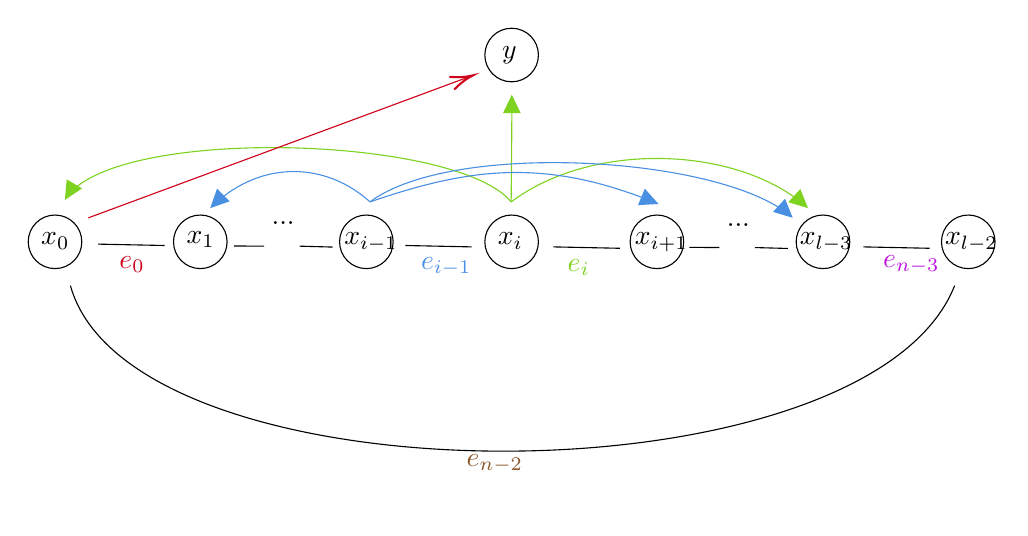
\begin{tikzpicture}[x=0.75pt,y=0.75pt,yscale=-1,xscale=1]
%uncomment if require: \path (0,300); %set diagram left start at 0, and has height of 300

%Shape: Circle [id:dp6772890116560196] 
\draw   (270,162.91) .. controls (270,155.78) and (275.78,150) .. (282.91,150) .. controls (290.03,150) and (295.81,155.78) .. (295.81,162.91) .. controls (295.81,170.03) and (290.03,175.81) .. (282.91,175.81) .. controls (275.78,175.81) and (270,170.03) .. (270,162.91) -- cycle ;
%Shape: Circle [id:dp5871526391848064] 
\draw   (420,162.91) .. controls (420,155.78) and (425.78,150) .. (432.91,150) .. controls (440.03,150) and (445.81,155.78) .. (445.81,162.91) .. controls (445.81,170.03) and (440.03,175.81) .. (432.91,175.81) .. controls (425.78,175.81) and (420,170.03) .. (420,162.91) -- cycle ;
%Shape: Circle [id:dp07729495910565454] 
\draw   (490,162.91) .. controls (490,155.78) and (495.78,150) .. (502.91,150) .. controls (510.03,150) and (515.81,155.78) .. (515.81,162.91) .. controls (515.81,170.03) and (510.03,175.81) .. (502.91,175.81) .. controls (495.78,175.81) and (490,170.03) .. (490,162.91) -- cycle ;
%Shape: Circle [id:dp262131491828823] 
\draw   (200,162.91) .. controls (200,155.78) and (205.78,150) .. (212.91,150) .. controls (220.03,150) and (225.81,155.78) .. (225.81,162.91) .. controls (225.81,170.03) and (220.03,175.81) .. (212.91,175.81) .. controls (205.78,175.81) and (200,170.03) .. (200,162.91) -- cycle ;
%Straight Lines [id:da10861800407645683] 
\draw    (231.67,164.68) -- (263.67,165.35) ;
%Straight Lines [id:da536121074656983] 
\draw    (368.48,165.57) -- (383,165.67) ;
%Straight Lines [id:da7967913679803297] 
\draw    (400.15,165.67) -- (416,166.11) ;
%Shape: Circle [id:dp6503647512544207] 
\draw   (120,162.91) .. controls (120,155.78) and (125.78,150) .. (132.91,150) .. controls (140.03,150) and (145.81,155.78) .. (145.81,162.91) .. controls (145.81,170.03) and (140.03,175.81) .. (132.91,175.81) .. controls (125.78,175.81) and (120,170.03) .. (120,162.91) -- cycle ;
%Shape: Circle [id:dp06282722717729516] 
\draw   (50,162.91) .. controls (50,155.78) and (55.78,150) .. (62.91,150) .. controls (70.03,150) and (75.81,155.78) .. (75.81,162.91) .. controls (75.81,170.03) and (70.03,175.81) .. (62.91,175.81) .. controls (55.78,175.81) and (50,170.03) .. (50,162.91) -- cycle ;
%Straight Lines [id:da6634256240143169] 
\draw    (83.67,164.02) -- (115.67,164.68) ;
%Straight Lines [id:da9040406415564918] 
\draw    (149.15,164.91) -- (163.67,165) ;
%Straight Lines [id:da7188137218222393] 
\draw    (180.81,165) -- (196.67,165.44) ;
%Shape: Circle [id:dp7453527750909341] 
\draw   (340,162.91) .. controls (340,155.78) and (345.78,150) .. (352.91,150) .. controls (360.03,150) and (365.81,155.78) .. (365.81,162.91) .. controls (365.81,170.03) and (360.03,175.81) .. (352.91,175.81) .. controls (345.78,175.81) and (340,170.03) .. (340,162.91) -- cycle ;
%Straight Lines [id:da6151250731140607] 
\draw    (303,165.35) -- (335,166.02) ;
%Straight Lines [id:da38307478583040533] 
\draw    (452.33,165.35) -- (484.33,166.02) ;
%Shape: Circle [id:dp9073302596091972] 
\draw   (270,72.91) .. controls (270,65.78) and (275.78,60) .. (282.91,60) .. controls (290.03,60) and (295.81,65.78) .. (295.81,72.91) .. controls (295.81,80.03) and (290.03,85.81) .. (282.91,85.81) .. controls (275.78,85.81) and (270,80.03) .. (270,72.91) -- cycle ;
%Curve Lines [id:da6936501442548073] 
\draw    (70.33,184.02) .. controls (99.67,290.02) and (454.33,290.68) .. (496.33,184.02) ;
%Curve Lines [id:da014900277525460415] 
\draw [color={rgb, 255:red, 126; green, 211; blue, 33 }  ,draw opacity=1 ]   (282.67,143.67) .. controls (321.87,114.27) and (390.52,116.91) .. (423.68,144.94) ;
\draw [shift={(425.67,146.68)}, rotate = 222.52] [fill={rgb, 255:red, 126; green, 211; blue, 33 }  ,fill opacity=1 ][line width=0.08]  [draw opacity=0] (8.93,-4.29) -- (0,0) -- (8.93,4.29) -- cycle    ;
%Curve Lines [id:da8694063449774041] 
\draw [color={rgb, 255:red, 126; green, 211; blue, 33 }  ,draw opacity=1 ]   (282.67,143.67) .. controls (282.97,114.26) and (283,104.99) .. (283,95.02) ;
\draw [shift={(283,92.02)}, rotate = 90] [fill={rgb, 255:red, 126; green, 211; blue, 33 }  ,fill opacity=1 ][line width=0.08]  [draw opacity=0] (8.93,-4.29) -- (0,0) -- (8.93,4.29) -- cycle    ;
%Curve Lines [id:da38542955546341706] 
\draw [color={rgb, 255:red, 126; green, 211; blue, 33 }  ,draw opacity=1 ]   (282.67,143.67) .. controls (256.86,112) and (95.64,106.88) .. (69.12,140.57) ;
\draw [shift={(67.67,142.68)}, rotate = 300.65] [fill={rgb, 255:red, 126; green, 211; blue, 33 }  ,fill opacity=1 ][line width=0.08]  [draw opacity=0] (8.93,-4.29) -- (0,0) -- (8.93,4.29) -- cycle    ;
%Curve Lines [id:da14735042368726803] 
\draw [color={rgb, 255:red, 74; green, 144; blue, 226 }  ,draw opacity=1 ]   (214.67,143.67) .. controls (253.87,114.27) and (380.78,121.39) .. (416.28,149.6) ;
\draw [shift={(418.33,151.35)}, rotate = 222.52] [fill={rgb, 255:red, 74; green, 144; blue, 226 }  ,fill opacity=1 ][line width=0.08]  [draw opacity=0] (8.93,-4.29) -- (0,0) -- (8.93,4.29) -- cycle    ;
%Curve Lines [id:da2490603722840098] 
\draw [color={rgb, 255:red, 74; green, 144; blue, 226 }  ,draw opacity=1 ]   (214.67,143.67) .. controls (261.62,127.59) and (297.9,122.18) .. (351.22,143.68) ;
\draw [shift={(353.67,144.68)}, rotate = 202.52] [fill={rgb, 255:red, 74; green, 144; blue, 226 }  ,fill opacity=1 ][line width=0.08]  [draw opacity=0] (8.93,-4.29) -- (0,0) -- (8.93,4.29) -- cycle    ;
%Curve Lines [id:da36788092610899037] 
\draw [color={rgb, 255:red, 74; green, 144; blue, 226 }  ,draw opacity=1 ]   (214.67,143.67) .. controls (193.65,124.61) and (162.91,123.41) .. (139.79,144.65) ;
\draw [shift={(137.67,146.68)}, rotate = 315] [fill={rgb, 255:red, 74; green, 144; blue, 226 }  ,fill opacity=1 ][line width=0.08]  [draw opacity=0] (8.93,-4.29) -- (0,0) -- (8.93,4.29) -- cycle    ;
%Straight Lines [id:da6908283822718694] 
\draw [color={rgb, 255:red, 208; green, 2; blue, 27 }  ,draw opacity=1 ][fill={rgb, 255:red, 208; green, 2; blue, 27 }  ,fill opacity=1 ]   (79,151.35) -- (262.46,83.38) ;
\draw [shift={(264.33,82.68)}, rotate = 159.67] [color={rgb, 255:red, 208; green, 2; blue, 27 }  ,draw opacity=1 ][line width=0.75]    (10.93,-3.29) .. controls (6.95,-1.4) and (3.31,-0.3) .. (0,0) .. controls (3.31,0.3) and (6.95,1.4) .. (10.93,3.29)   ;

% Text Node
\draw (420.5,157.4) node [anchor=north west][inner sep=0.75pt]    {$x_{l-3}$};
% Text Node
\draw (275,157.4) node [anchor=north west][inner sep=0.75pt]    {$x_{i}$};
% Text Node
\draw (490.5,157.4) node [anchor=north west][inner sep=0.75pt]    {$x_{l-2}$};
% Text Node
\draw (201,157.4) node [anchor=north west][inner sep=0.75pt]    {$x_{i-1}$};
% Text Node
\draw (238,169.4) node [anchor=north west][inner sep=0.75pt]  [color={rgb, 255:red, 74; green, 144; blue, 226 }  ,opacity=1 ]  {$e_{i-1}{}$};
% Text Node
\draw (460.67,168.07) node [anchor=north west][inner sep=0.75pt]  [color={rgb, 255:red, 189; green, 16; blue, 224 }  ,opacity=1 ]  {$e_{n-3}{}$};
% Text Node
\draw (385.33,152.67) node [anchor=north west][inner sep=0.75pt]   [align=left] {...};
% Text Node
\draw (125,156.73) node [anchor=north west][inner sep=0.75pt]    {$x_{1}$};
% Text Node
\draw (55,157.4) node [anchor=north west][inner sep=0.75pt]    {$x_{0}$};
% Text Node
\draw (166,152) node [anchor=north west][inner sep=0.75pt]   [align=left] {...};
% Text Node
\draw (341,157.4) node [anchor=north west][inner sep=0.75pt]    {$x_{i+1}$};
% Text Node
\draw (308.67,170.07) node [anchor=north west][inner sep=0.75pt]  [color={rgb, 255:red, 126; green, 211; blue, 33 }  ,opacity=1 ]  {$e_{i}{}$};
% Text Node
\draw (92.67,168.73) node [anchor=north west][inner sep=0.75pt]  [color={rgb, 255:red, 208; green, 2; blue, 27 }  ,opacity=1 ]  {$e_{0}{}$};
% Text Node
\draw (277,67.4) node [anchor=north west][inner sep=0.75pt]    {$y$};
% Text Node
\draw (260,264.07) node [anchor=north west][inner sep=0.75pt]  [color={rgb, 255:red, 139; green, 87; blue, 42 }  ,opacity=1 ]  {$e_{n-2}{}$};

\end{tikzpicture}


\captionof{figure}{Representation of digraph $A(D)$. Each colored edge belongs to the digraph.}
\end{center}

Observe that as $\delta(G_i) \geq \frac{n}{2}$ for all $i \in \{0, \dots, n - 2\}$, thus 
$d^+_{D}(x) \geq \frac{n}{2} - 1$ for every vertex $x$ on the cycle. We get that 
$|A(D)| \geq (n-1)(\frac{n}{2} - 1)$. 

Now, let's define the following variables:

\begin{itemize}
    \item $in\_degree$: An array of size $n$ where $in\_degree[i]$ is the in-degree of vertex $i$ in the digraph $D$.
    \item $incoming\_neighborhood$: An array of size $n$ where $incoming\_neighborhood[i]$ is the list of vertices that have an edge to vertex $i$ in the digraph $D$.
    \item $I \coloneqq \{i \in [n - 1]: \{x_i, y\} \in A(D)\}$
    \item $\bar{I} \coloneqq \{i \in [n - 1]: edge(y, x_{i+1}, cy) \in E(G)\}$
\end{itemize}

To effectively build these variables, we can iterate over the vertices of the cycle and iterate over it's adjacency list,
such as the following algorithm:

\begin{algorithm}[H]
    \caption{Part 2: Cycle Extension for \( l < n - 1 \). Building digraph variables, $I$ and $\bar{I}$}
    \begin{algorithmic}[1]
        \Function{Extend\_Cycle}{$G, C$}
            \State $I \gets []$
            \State $in\_degree \gets [0] \times n$
            \State $incoming\_neighborhood \gets [\text{empty list}] \times n$
            
            \For{$i \gets 0$ to $cycle\_size - 1$}
                \State $u \gets cycle.vertices[i]$
                \State $v \gets cycle.vertices[(i + 1) \bmod cycle\_size]$
                \State $color \gets color\_in\_position[i]$
                
                \For{$tgt \in G.adjacency[color][u]$}
                    \If{$tgt = v$}
                        \State \textbf{continue}
                    \EndIf
                    
                    \State $in\_degree[tgt] \gets in\_degree[tgt] + 1$
                    \State $incoming\_neighborhood[tgt].append(u)$
                    
                    \If{$tgt = y$}
                        \State $I.append(i)$
                    \EndIf
                \EndFor
            \EndFor
            
            \State $\bar{I} \gets \text{Find\_Adjacency}(y, cy, vertex\_position\_on\_cycle)$
            \State $\bar{I} \gets [(u - 1 + cycle\_size) \bmod cycle\_size : u \in \bar{I}]$

        \EndFunction
    \end{algorithmic}
\end{algorithm}

The complexity of this algorithm is $O(n^2)$, as we need to iterate over the vertices of the cycle and iterate over 
it's adjacency list for a specific color. 

Let's find the answer for the case $d^-_D(y) \geq \frac{n}{2}$. We have that 
$|I| + |\bar{I}|  \geq d^-_D(y) +  \frac{n}{2} $. 
Thus, from Dirichlet Principle, $I \cap \bar{I} \neq \emptyset$. In this case, we can build 
a cycle of length $n$ with the following crossing, removing the edge $x_i$:

% set scale
\begin{figure}[H]
    \centering
    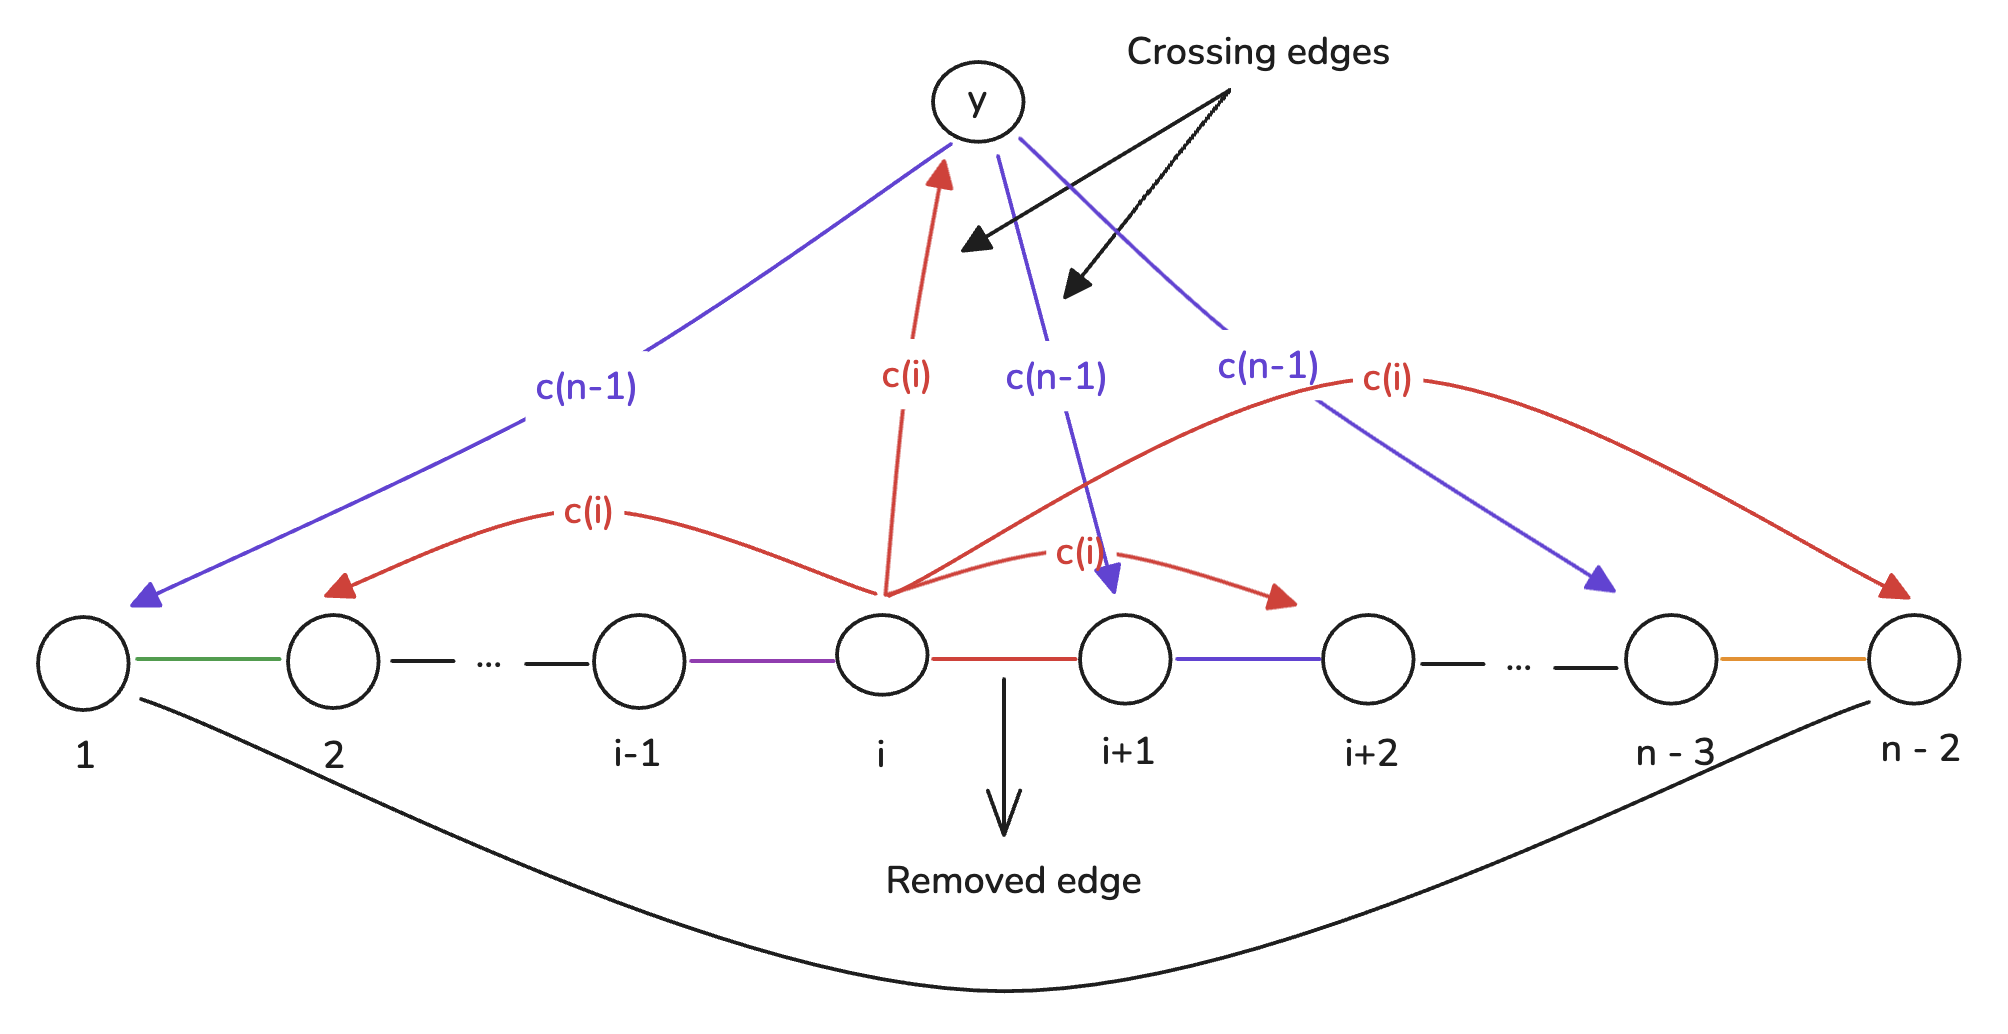
\includegraphics[width=1\textwidth]{figuras/cycle_n-1_crossing_1.png}
    \caption{Crossing for the case $d^-_D(y) \geq \frac{n}{2}$.}
    \label{fig:crossing_case_2}
\end{figure}

To the algorithm part, we can just check the intersection and build the answer.

\begin{algorithm}[H]
    \caption{Part 3: Cycle Extension for \( l < n - 1 \). Case \( d^-_D(y) \geq \frac{n}{2} \)}
    \begin{algorithmic}[1]
        \Function{Extend\_Cycle}{$G, C$}
            \For{$i \in I$}
                \If{$i \in \bar{I}$}
                    \State \Return \Call{Find\_Answer}{$G, y, cy, C, i$}
                \EndIf
            \EndFor
        \EndFunction
    \end{algorithmic}
\end{algorithm}

The complexity is $O(n^2)$, as we just need to iterate over $I$, check if it's in $\bar{I}$ and, once we find an element in $\bar{I}$, 
we call the function \texttt{Find\_Answer} that has complexity $O(n)$.

From now on, we will assume that $d^-_D(y) < \frac{n}{2}$. Here we will divide in two cases:

\begin{enumerate}
    \item If there is a vertex $x_i$ such that $d^-_D(x_i) > \frac{n}{2} - 1$.
    \item Otherwise.
\end{enumerate}

Let's start with the first case. We may assume, WLOG, that $d^-_D(x_0) > \frac{n}{2} - 1$.
For this, we can just find the vertex $x_i$ and rotate the cycle, such as the following algorithm:

\begin{algorithm}[H]
    \caption{Part 4: Cycle Extension for \( l < n - 1 \). Case \( d^-_D(y) < \frac{n}{2} \)}
    \begin{algorithmic}[1]
        \Function{Extend\_Cycle}{$G, C$}
            \For{$i \in [0, \dots, cycle\_size - 1]$}
                \State $u \gets cycle.vertices[i]$
                \If{$in\_degree[u] > \frac{n}{2} - 1$}
                    \State $cycle.vertices \gets cycle.vertices[i:] + cycle.vertices[:i]$
                    \State $cycle.edges \gets cycle.edges[i:] + cycle.edges[:i]$
                \EndIf
                % # Rebuild the needed variables
                \For{$j \in [0, \dots, cycle\_size - 1]$}
                    \State $color \gets cycle.edges[j].color$
                    \State $new\_color\_id[color] \gets j$
                    \State $vertex\_position\_on\_cycle[cycle.vertices[j]] \gets j$
                    \State $pos\_color\_cic[j] \gets color$
                \EndFor
                \State \textbf{break}
            \EndFor
        \EndFunction
    \end{algorithmic}
\end{algorithm}

The time completity for this is just $O(n)$, as we iterate over the vertices and
as soon as we find a vertex with in-degree greater than $\frac{n}{2} - 1$, we make 
$O(n)$ operations to rebuild the needed variables and then we break.

Let's define the following variables:

\begin{itemize}
    \item $I_0 \coloneqq \{i \in [n - 1]: edge(x_i, y, c_0) \in E(G)\}$
    \item $I_{n-1} \coloneqq \{i \in [n - 1]: edge(x_{i+1}, y, c_{n-1}) \in E(G)\}$
\end{itemize}

We have that $I_0 + I_{n-1} \geq d_{G_0}(y) + d_{G_{n-1}}(y) \geq n$. Thus, 
from Dirichlet Principle, $I_0 \cap I_{n-1} \neq \emptyset$. Take $j \in I_0 \cap I_{n-1}$.
If $j = 0$, we can just remove the edge $x_0$ and build the cycle of length $n$ 
adding crossing edges $edge(x_0, y, c_0)$ and $edge(y, x_1, c_1)$. So, assume $j \neq 0$.

Let's construct a $G$-transversal path $P$ such as on the figure below:

\begin{figure}[H]
    \centering
    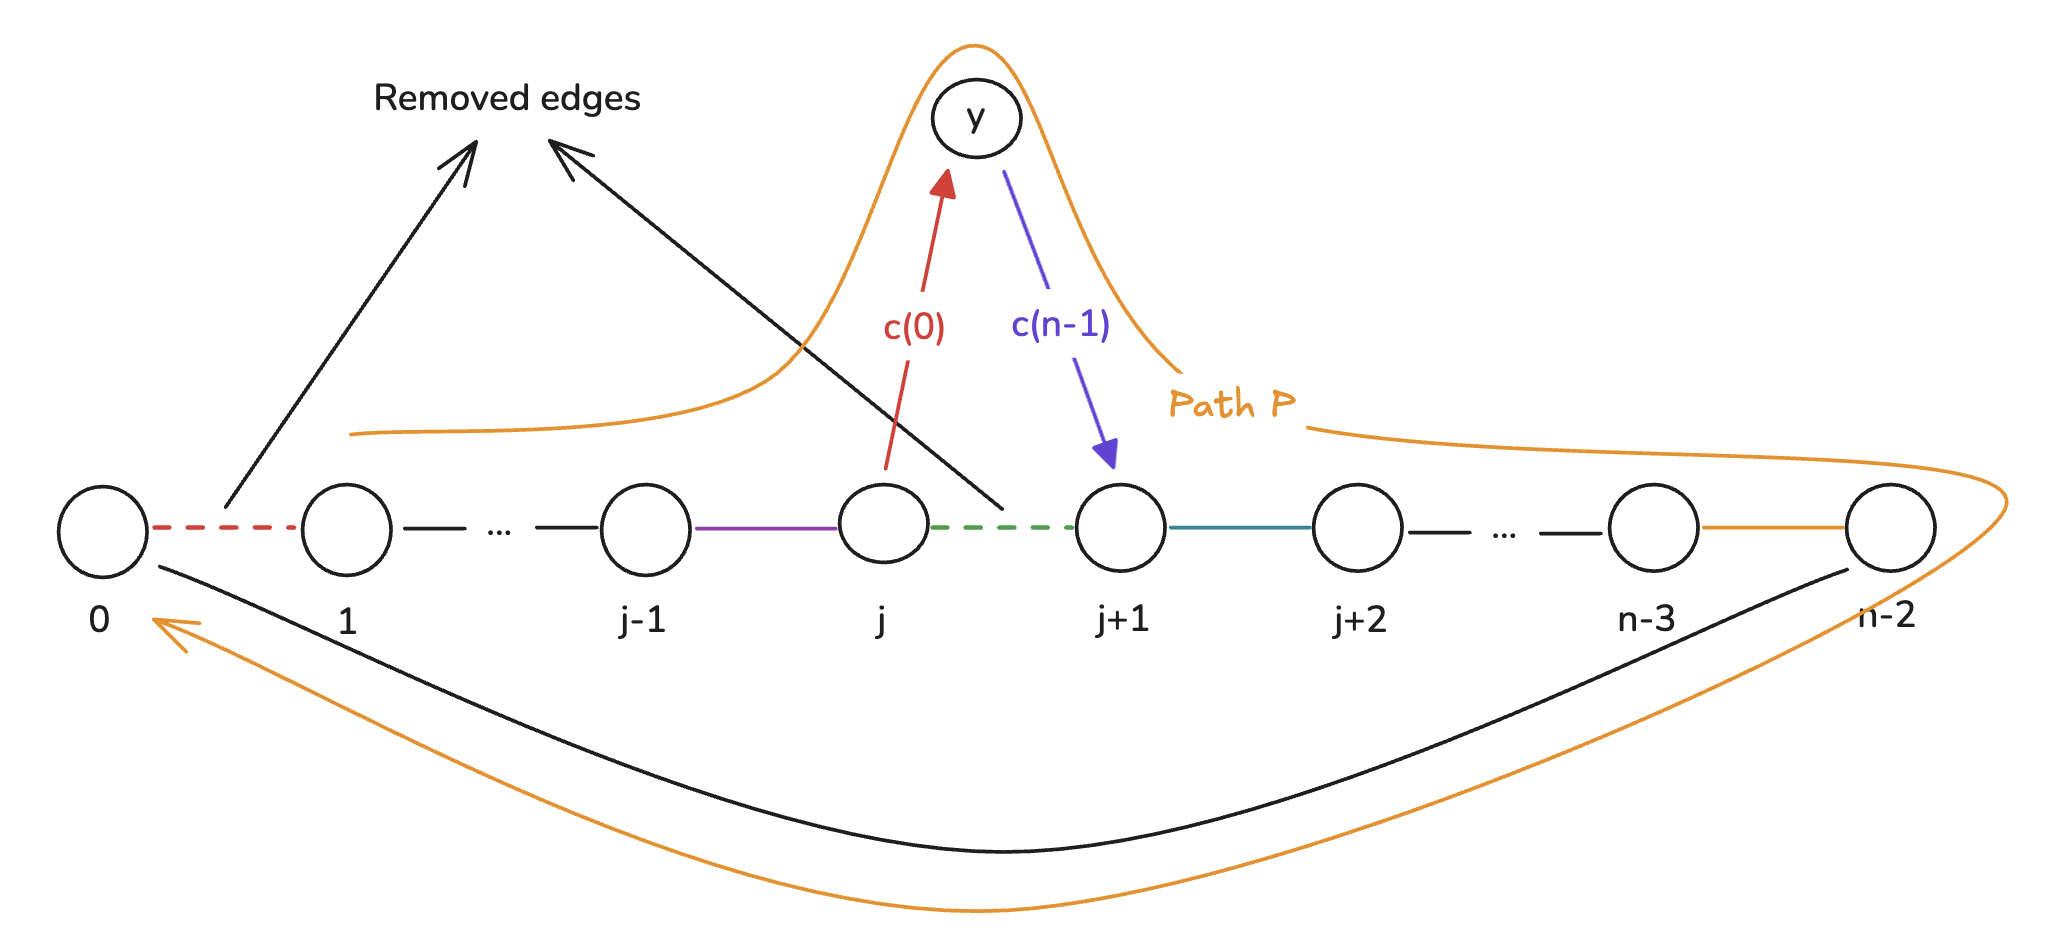
\includegraphics[width=1\textwidth]{figuras/cycle_n-1_build_path.png}
    \caption{Building the transversal path $P$.}
    \label{fig:cycle_n-1_build_path}
\end{figure}

We are going to create the following variables to manipulate the path $P$:

\begin{itemize}
    \item $removed\_color$: The color of the edge outside the path $P$, $C.edges[j].color$;
    \item $P\_vertices$: The vertices of the path $P$, $(x_1, x_2, \dots, x_{j}, y, x_{j+1}, \dots, x_{n-2}, x_{0})$;
    \item $P\_edges$: The edges of the path $P$, $(e_1, e_2, \dots, e_{j}, e_{j+1}, \dots, e_{n-2}, e_{0})$;
    \item $P\_pos$: An array to store the new position of each vertex on the path.
\end{itemize}

To compute these variables, we can use the following algorithm:
\begin{algorithm}[H]
    \caption{Part 5: Cycle Extension for \( l < n - 1 \). Case \( d^-_D(y) < \frac{n}{2} \)}
    \begin{algorithmic}[1]
        \Function{Extend\_Cycle}{$G, C$}
            \State $j \gets -1$
            \State $removed\_color \gets -1$
            \State $P\_vertices \gets []$
            \State $P\_edges \gets []$
            \State $P\_pos \gets [0] \times n$

            \For{$i \in I_0$}
                \If{$i \in I_{n-1}$}
                    \If{$i = 0$}
                        \State \Return \Call{Find\_Answer}{$G, y, cy, C, i$}
                    \EndIf

                    \State $j \gets i$

                    \State $removed\_color \gets C.edges[j].color$
                    \State $P\_vertices \gets C.vertices[1:j+1] +$
                    \State $\hspace{4.3em} \gets [y] +$
                    \State $\hspace{4.3em} \gets C.vertices[j+1:n] +$
                    \State $\hspace{4.3em} \gets [C.vertices[0]]$

                    \State $P\_edges \gets C.edges[1:j] +$
                    \State $\hspace{4.1em} \gets [G.get\_edge(C.vertices[j], y, pos\_color\_cic[0])] +$
                    \State $\hspace{4.1em} \gets [G.get\_edge(y, C.vertices[(j + 1) \bmod n], cy)] +$
                    \State $\hspace{4.1em} \gets C.edges[j+1:n]$

                    \For{$j \in [0, \dots, n-1]$}
                        \State $P\_pos[P\_vertices[j]] \gets j$
                    \EndFor

                    \State \textbf{break}
                \EndIf
            \EndFor
        \EndFunction
    \end{algorithmic}
\end{algorithm}

The time complexity is $O(n^2)$, as we iterate over $I_0$, check if it's in $I_{n-1}$ and, if it is, we build the path $P$ just once.
To build the path it is just $O(n)$ operations.

Let's now create the following variables:

\begin{itemize}
    \item $J_0 \coloneqq \{i \in [n-2]: edge(P\_vertices[0], P\_vertices[i + 1], removed\_color) \in E(G)\}$
    \item $J_{n-1} \coloneqq \{i \in [n-2]: P\_vertices[i] \in incoming\_neighborhood[P\_vertices[n - 1]]\}$
\end{itemize}


If $edge(P\_vertices[0], P\_vertices[-1], removed\_color)$ in $G$, we can just 
close the cycle adding this edge. Let's assume then we don't have this edge. 
Thus, $|J_0| \geq \delta(G_{removed\_color}) \geq \frac{n}{2}$. Also, as $P\_vertices[-2] \in \{x_{n-2}, y\}$, 
from the construction of $D$ we guarantee that $P\_vertices[n-2] \notin N^-_D(x_0)$
and consequently $|J_{n-1}| \geq \frac{n}{2} - \frac{1}{2}$.

From Dirichlet Principle, as $|J_0| + |J_{n-1}| \geq n$, we have that $|J_0 \cap J_{n-1}| \geq 2$. Thus,
there is at least one element on $J_0 \cap J_{n-1}$, let's call it $k$, such that $P\_vertices[k] \neq y$.
We can then build the following $G$-transversal cycle:

\begin{figure}[H]
    \centering
    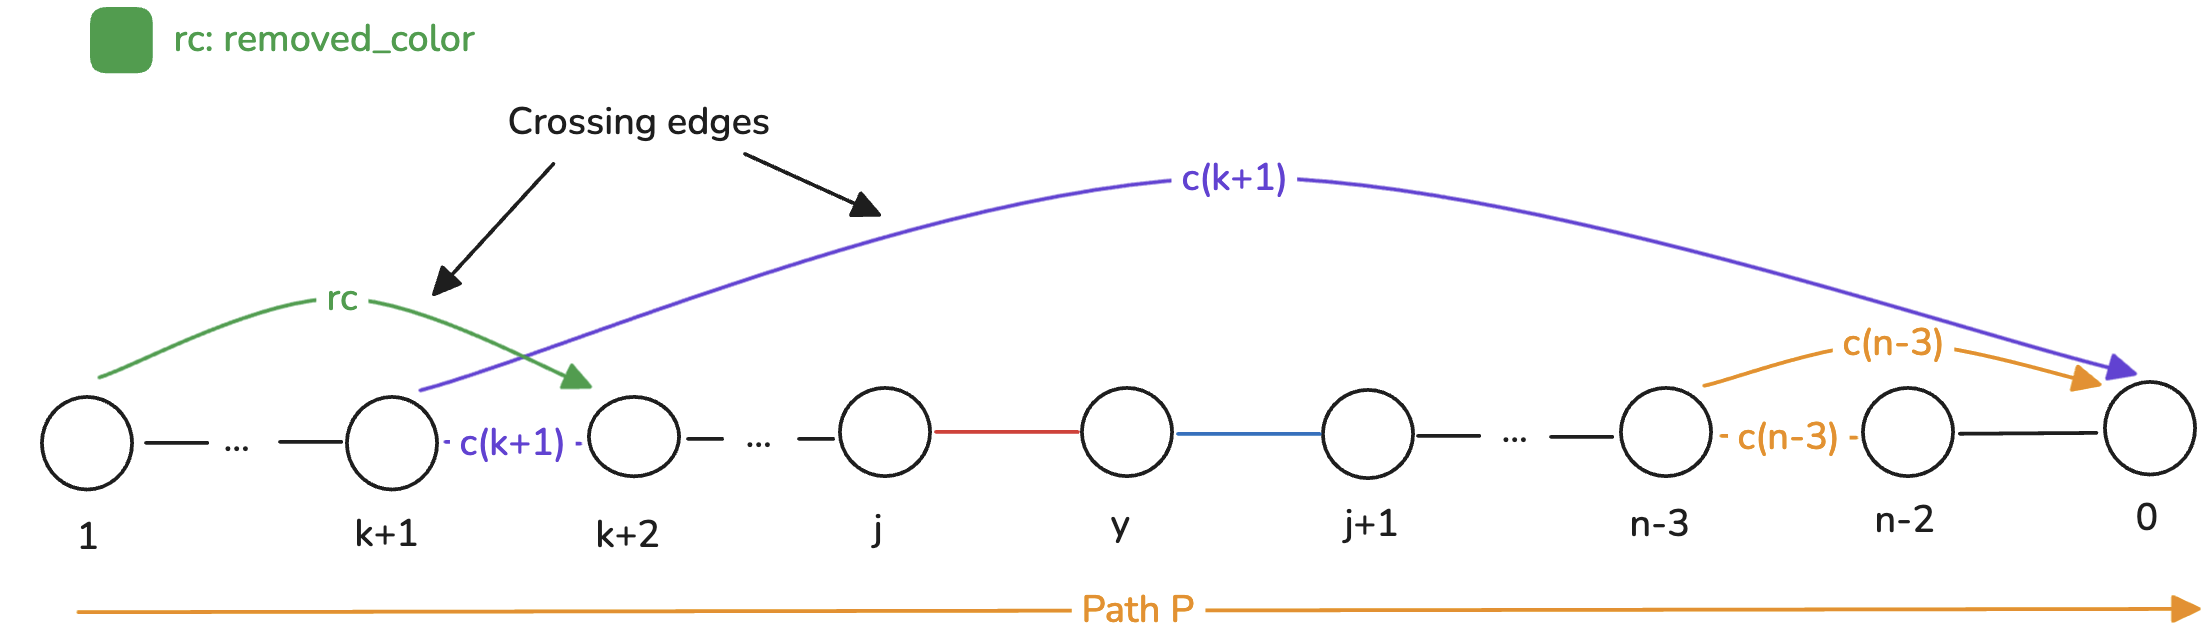
\includegraphics[width=1\textwidth]{figuras/cycle_n-1_cruzamento_not_y.png}
    \caption{Crossing for the case $d^-_D(y) < \frac{n}{2}$ and $P\_vertices[k] \neq y$.}
    \label{fig:cycle_n-1_cruzamento_not_y}
\end{figure}

The algorithm to find the answer in this case is the following:

\begin{algorithm}[H]
    \caption{Part 6: Cycle Extension for \( l < n - 1 \). Case \( d^-_D(y) < \frac{n}{2} \)}
    \begin{algorithmic}[1]
        \Function{Extend\_Cycle}{$G, C$}
            \State $edge \gets G.check\_edge(P\_vertices[0], P\_vertices[-1], removed\_color)$
            \If{$edge$ is not $None$}
                \State \Return \Call{Cycle}{$G, P\_vertices, P\_edges + [edge]$}
            \EndIf

            \State $J1 \gets \Call{Find\_Adjacency}{$P\_vertices[0], removed\_color, P\_pos$}$
            \State $J1 \gets [(u - 1 + n) \bmod n : u \in J1]$

            \State $Jn \gets incoming\_neighborhood[P\_vertices[-1]]$
            \State $Jn \gets [P\_pos[u] : u \in Jn]$

            \For{$i \in J1$}
                \If{$i \in Jn$}
                    \If{$P\_vertices[i + 1] = y$}
                        \State \textbf{continue}
                    \EndIf

                    \State $final\_vertices \gets P\_vertices[:i+1] + P\_vertices[i+1:][::-1]$
                    \State $final\_edges \gets P\_edges[:i] +$
                    \State $\hspace{6.7em} [G.get\_edge(P\_vertices[i], P\_vertices[-1], P\_edges[i].color)] +$
                    \State $\hspace{6.7em} P\_edges[i+1:][::-1] +$
                    \State $\hspace{6.7em} [G.get\_edge(P\_vertices[i+1], P\_vertices[0], removed\_color)]$

                    \State \Return \Call{Cycle}{$G, final\_vertices, final\_edges$}
                \EndIf
            \EndFor
        \EndFunction
    \end{algorithmic}
\end{algorithm}

The time complexity is $O(n^2)$, as we iterate over $J_0$ and check 
if the element is in $J_{n-1}$. If it is, we build the cycle and return it, in $O(n)$ operations.
Therefore, for the there exists $x_i$ such that $d^-_D(x_i) > \frac{n}{2} - 1$, we have a total 
complexity of $O(n^2)$.

Now, let's analyze the case where every $x_i$ satisfies $d^-_D(x_i) \leq \frac{n}{2} - 1$.

\pagestyle{mainmatter}
\input{conteudo/04-ore-therorem}


%%%%%%%%%%%%%%%%%%%%%%%%%%%% APÊNDICES E ANEXOS %%%%%%%%%%%%%%%%%%%%%%%%%%%%%%%%

%%%%%%%%%%%%%%% SEÇÕES FINAIS (BIBLIOGRAFIA E ÍNDICE REMISSIVO) %%%%%%%%%%%%%%%%

\backmatter
\pagestyle{backmatter}
\addtocontents{toc}{\vspace{2\baselineskip plus .5\baselineskip minus .5\baselineskip}}
\printbibliography[
  title=\refname\label{sec:bib}, % "Referências", recomendado pela ABNT
  title=\bibname\label{sec:bib}, % "Bibliografia"
  heading=bibintoc, % Inclui a bibliografia no sumário
]

\end{document}
